\documentclass{article}
\textheight 23.5cm \textwidth 15.8cm
%\leftskip -1cm
\topmargin -1.5cm \oddsidemargin 0.3cm \evensidemargin -0.3cm
%\documentclass[final]{siamltex}

\usepackage{verbatim}
\usepackage{fancyhdr}
\usepackage{amssymb,ctex}
\usepackage{mathrsfs}
\usepackage{latexsym,amsmath,amssymb,amsfonts,epsfig,graphicx,cite,psfrag}
\usepackage{eepic,color,colordvi,amscd}
\usepackage{enumerate}
\usepackage{booktabs}
\usepackage{graphicx}
\usepackage{float}
\usepackage{multirow}


\title{Numerical Analysis Homework10}
\author{Zhang Jiyao,PB20000204}

\begin{document}
	\maketitle
	
	\section{Introduction}
   
   画出五阶\text{Adams-Bashforth}公式和五阶\text{Adams-Moulton}公式的绝对稳定性区域,可以使用\text{Mathematica}绘制。

	\section{Method}
	
	多步方法的绝对稳定性:若差分方程作用到微分方程
	$$ \frac{dy}{dx}=\lambda y.(Re\lambda <0)$$
	
	时,对任意的初值,总存在左半复平面上的一个区域,当$\lambda h$在这个区域时,差分方程的解趋于0,这个区域称为稳定区域。
	
	即为复数$\omega$的集合,它使得$p-\omega q$的根位于单位圆盘内部。
	
	基于等距节点$t_i=x_0+ih(1\leq i \leq n)$的五阶\text{Adams-Bashforth}公式为:
	$$ x_{n+1}=x_n+\frac{h}{720}[1901f_n-2774f_{n-1}+2616f_{n-2}-1274f_{n-3}+251f_{n-4}]$$
	
	即有
	$$ x_{n+1}-x_n=\frac{h}{720}[1901f_n-2774f_{n-1}+2616f_{n-2}-1274f_{n-3}+251f_{n-4}]$$
	
	则有:
	$$ p(z)=z^5-z^4$$
	$$ q(z)=\frac{1}{720}[1901f_n-2774f_{n-1}+2616f_{n-2}-1274f_{n-3}+251f_{n-4}]$$
	
	则多项式$\phi=p-\lambda hq$为:
	$$ \phi=z^5+(-1-h\lambda \frac{1901}{720})z^4+(0+h\lambda \frac{2774}{720})z^3+(0-h\lambda \frac{2616}{720})z^2+(0+h\lambda \frac{1274}{720})z+(0-h\lambda \frac{251}{720})$$
	
	求$h\lambda$的值,使得多项式的根都落在单位圆盘内。
	
	基于等距节点$t_i=x_0+ih(1\leq i \leq n)$的五阶\text{Adams-Moulton}公式为:
	$$ x_{n+1}=x_n+\frac{h}{720}[251f_{n+1}+646f_{n}-264f_{n-1}+106f_{n-2}-19f_{n-3}]$$
	
	即有
	$$ x_{n+1}-x_n=\frac{h}{720}[251f_{n+1}+646f_{n}-264f_{n-1}+106f_{n-2}-19f_{n-3}]$$
	
	则有:
	$$ p(z)=z^4-z^3$$
	$$ q(z)=\frac{1}{720}[251f_{n+1}+646f_{n}-264f_{n-1}+106f_{n-2}-19f_{n-3}]$$
	
	则多项式$\phi=p-\lambda hq$为:
	$$ \phi=(-1-h\lambda \frac{251}{720})z^4+(-1-h\lambda \frac{646}{720})z^3+(0+h\lambda \frac{264}{720})z^2+(0-h\lambda \frac{106}{720})z+(0-h\lambda \frac{19}{720})$$
	
	求$h\lambda$的值,使得多项式的根都落在单位圆盘内。
	
	\section{Results}
	
		\begin{figure}[H]
		\begin{center}
			
			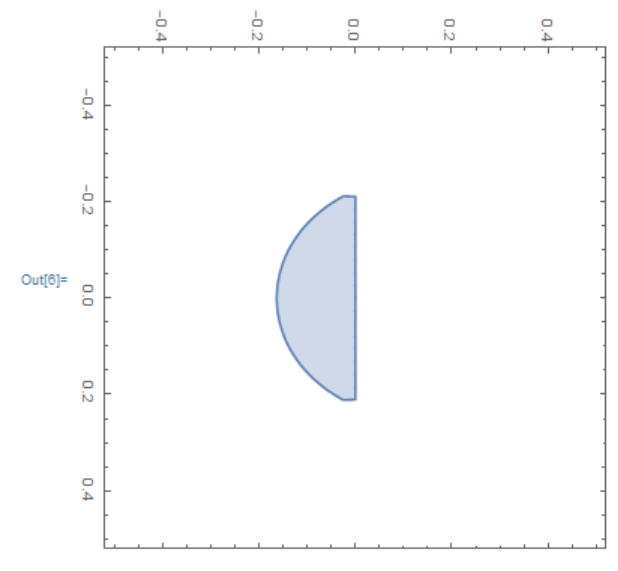
\includegraphics[width=5cm,height=5cm]{Bashforthgraph}
			
			\caption{Adams-Bashforth公式的图像} \label{Bashforthgraph.label}
		\end{center}
	\end{figure}
	
	\begin{figure}[H]
		\begin{center}
			
			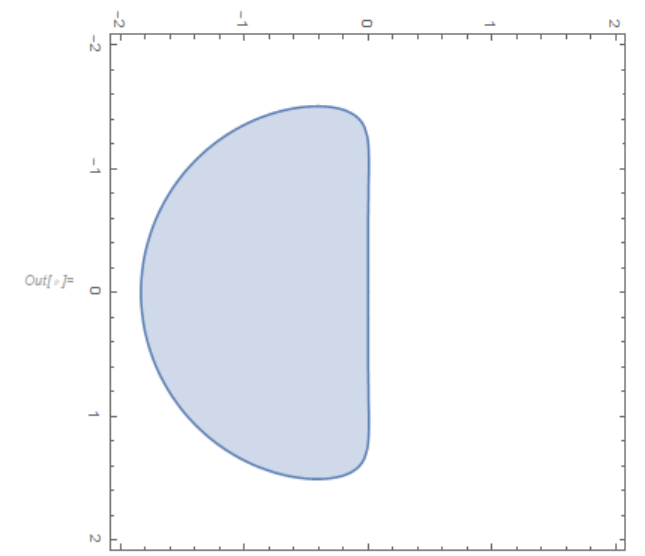
\includegraphics[width=5cm,height=5cm]{Moultongraph}
			
			\caption{Adams-Moulton公式的图像} \label{Moultongraph.label}
		\end{center}
	\end{figure}


	\section{Discussion}
	
    可以看到两个方法的绝对稳定性区域都是落在左半平面的。
	
	\section{Computer Code}
	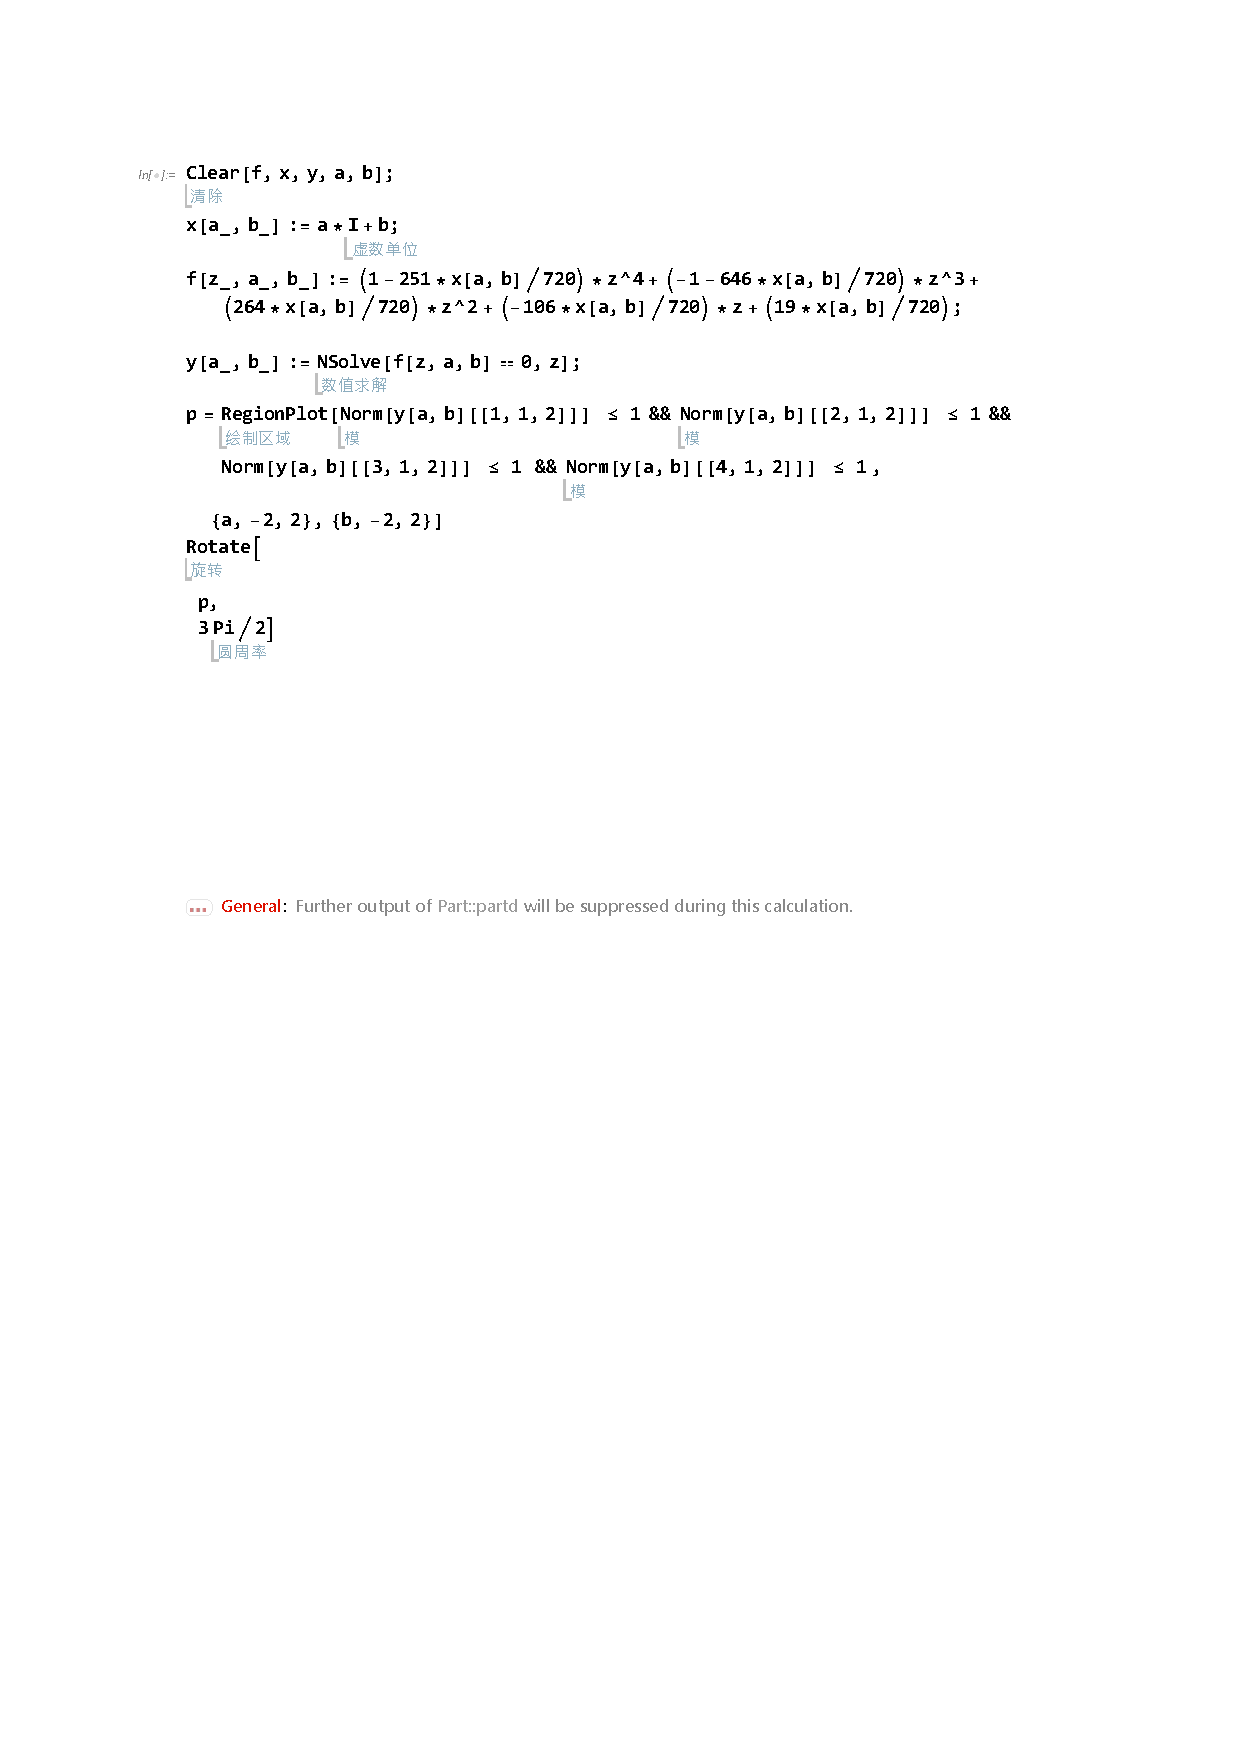
\includegraphics[width=\textwidth]{Moulton.pdf}
	
	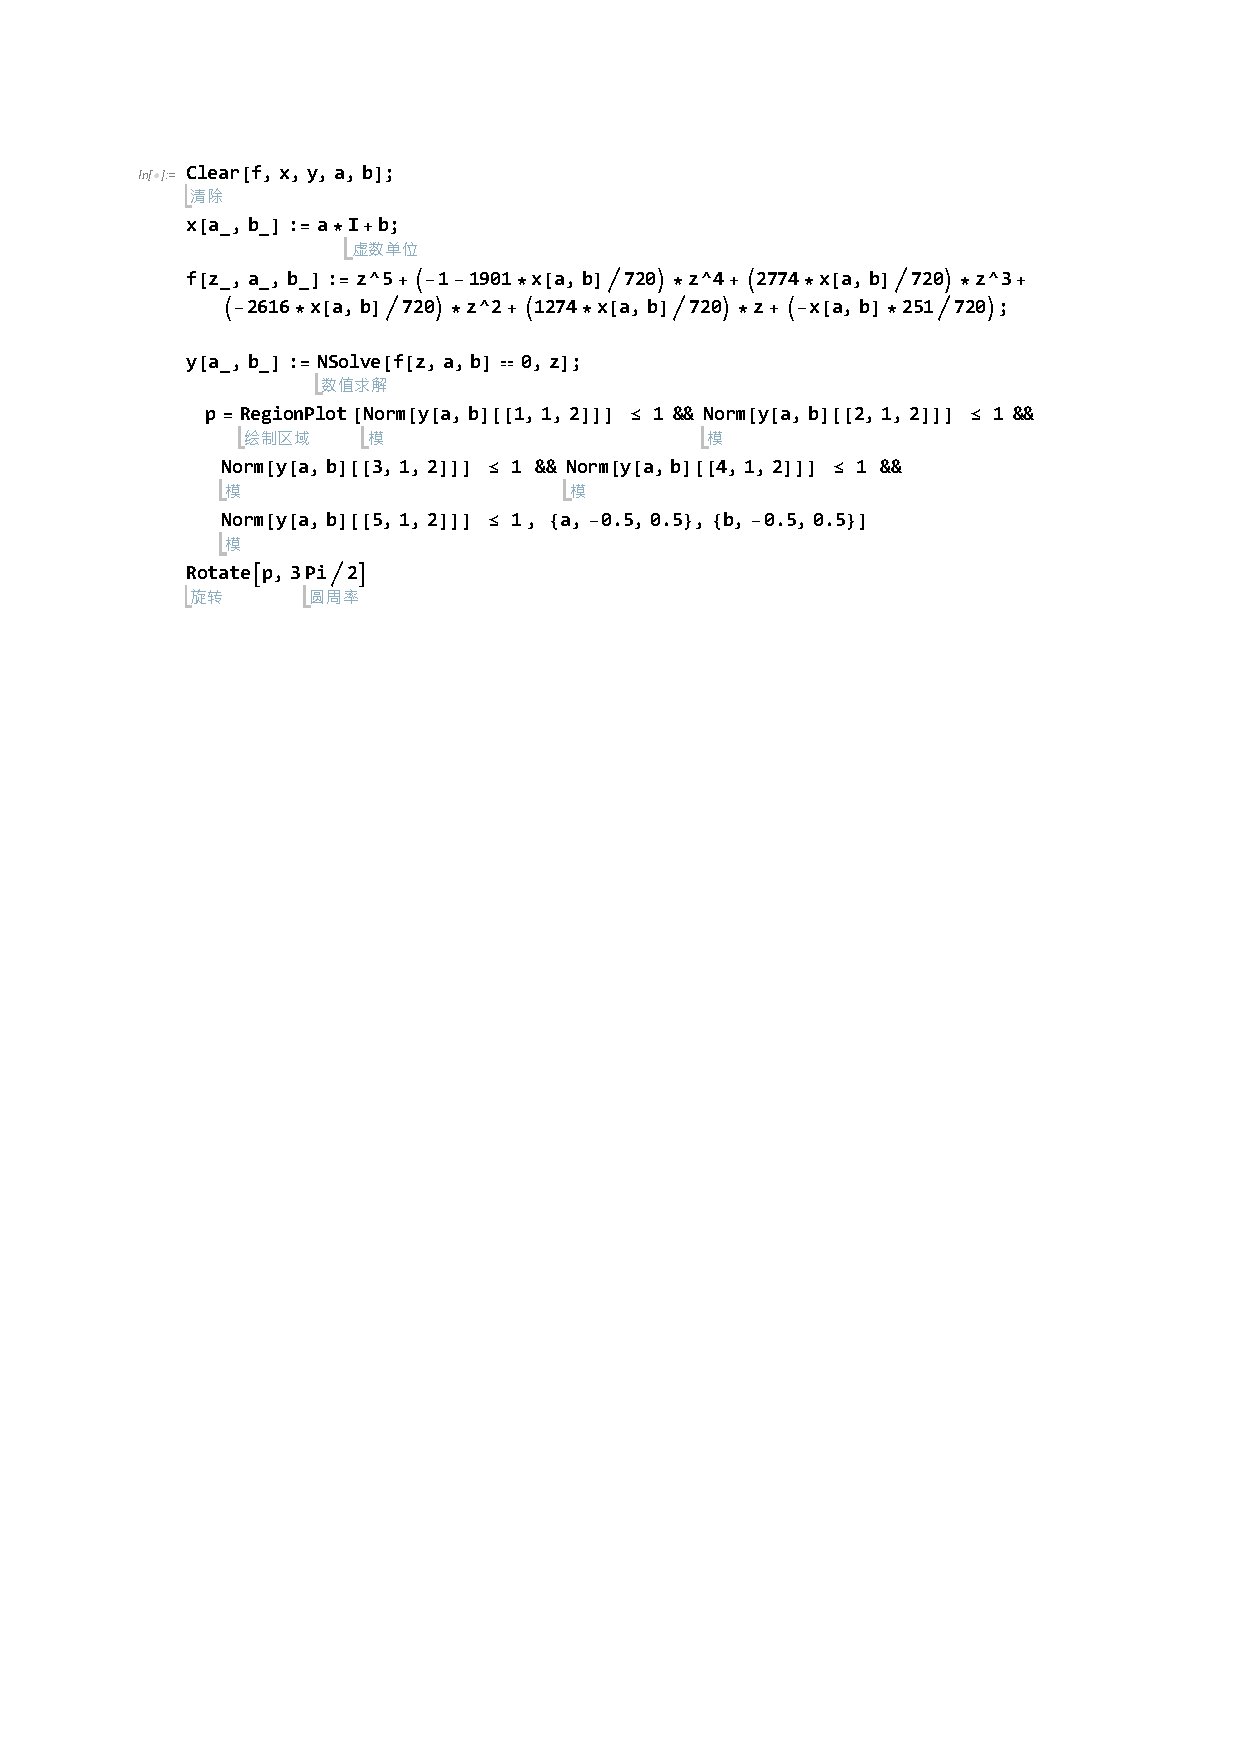
\includegraphics[width=\textwidth]{Bashforth.pdf}

\end{document}